%%
%% Author: Alexander
%% 18.02.2018
%%

% Preamble
\documentclass[a4paper,12pt]{article}

% Packages
\usepackage[14pt]{extsizes}
\usepackage{mathtext}
\usepackage[T2A]{fontenc}
\usepackage[utf8]{inputenc}
\usepackage[pdftex]{hyperref}
\usepackage[russian]{babel}
\usepackage{amsmath}
\usepackage{longtable}
\usepackage{amsfonts}
\usepackage{amssymb}
\usepackage{graphicx}
\usepackage[left=2cm,right=2cm,
    top=2cm,bottom=2cm,bindingoffset=0cm]{geometry}
\usepackage{color}
\usepackage{gensymb}
\linespread{1.25}

\usepackage{enumitem}
\setlist[enumerate]{label*=\arabic*.}

\usepackage{indentfirst}

\usepackage{titlesec}

% Document
\begin{document}

    \begin{titlepage}

        \begin{center}
            \begin{Large}
            МГТУ\ им.\ Н.Э.\ Баумана\\
            \end{Large}
            \begin{large}
            \vspace{6cm}
            Черновик диплома\\
            \vfill
            \end{large}
        \end{center}

        \begin{flushright}
            \begin{large}
            Жигалкин А.С.\\
            Группа: Э3-122\\
            \vspace{2cm}
            \end{large}
        \end{flushright}

        \begin{large}
            \begin{center}
           Москва\ 2018
            \end{center}
        \end{large}

    \end{titlepage}


    \tableofcontents
    \newpage

%	</ import '2N.tex' as TwoN />
%   </ import 'equipment.tex' as Equip/>
%   </ import 'turb_average_streamline.tex' as turb_avline_temp />
%   </ import 'comp_average_streamline.tex' as comp_avline_temp />
%   </ import 'turb_profiling.tex' as turb_prof_temp />
%   </ import 'turb_cooling.tex' as turb_cool_temp />
%   </ import 'comb_geom.tex' as comb_geom_templ/>


    \section{ВВЕДЕНИЕ}
    Газотурбинные имееют достаточно широкое примение в энергетике в качестве привода электрогенератора.
    Основными особенностями ГТУ по сравнению с энергетическими установками других типов являются:
    \begin{enumerate}
        \item Высокая маневренность.
        \item Компактность.
        \item Малый срок ввода в эксплуатацию.
        \item Низкая потребность в воде.
        \item Относительно низкий капитальные затраты.
        \item Относительно низкая экономичность.
        \item Относительно невысокая потребность в смазочных материалах (по сравнению с двигателями
        внутреннего сгорания)
    \end{enumerate}
    Данные особенности определяют основные области применения ГТУ.
    Они используются как правило для покрытия пиковых нагрузок в составе электростанций или для
    энергоснабжения промышленных предприятий, морских платформ, небольших населенных пунктов и т.п.
    Энергетических установок, которые обладали бы в перечисленных областях существенными преимуществами перед ГТУ, на
    данный момент не существует.
    Поэтому создание новых газотурбинных установок, обладающих большей экономичностью,
    меньшими капитальными затратами, большей материалоемкостью, чем существующие, является актуальной задачей.
    В данной выпускной квалификационной работе эта задача будет решаться для класса мощности 16 МВт.

    Проектируемая ГТУ будет обладать большей, чем у конкурентов, начальной температурой газа в цикле
    ($ << comb_chamber.T_stag_out >>\ К $).
    Это потребует проектирования более совершенной системы охлаждения, но позволит добится большей экономичности и
    меньшей металлоёмкостью, за счет возможности уменьшить диаметральный размер лопаточных машин.
    Установка будет выполнена по двухвальной схеме со свободной турбиной.
    Энергоблок на основе ГТУ будет выполнен по модульному принципу, что обеспечит удобство транспортировки установки с
    завода-изготовителя и высокую скорость строительства блока.

    \newpage

    \section{Техническое задание на диплом.}
    Спроектировать газотурбинную установку мощностью 16 МВт, предназначенную для
    привода электрогенератора.
    Топливо - природный газ.

    \newpage

    \section{Обоснование выбора схемы и параметров ГТУ.}

    \subsection{Обзор существующих энергетических приводных ГТУ в классе мощности 16 МВт.}

     Ниже будут рассмотрены следующие ГТУ энергетического назначения в классе мощность 16 МВт:
    \begin{enumerate}
        \item Установка ГТЭ-16ПА фирмы АО «ОДК-Пермские моторы».
        \item Установка SGT-500 фирмы Siemens.
        \item УстановкаTitan 130 фирмы Solar Turbines Inc.
        \item Установка АЛ-31СТЭ фирмы ПАО «ОДК-УМПО».
        \item Установка Т16 фирмы АО «РЭП Холдинг».
    \end{enumerate}

    \paragraph{Установка ГТЭ-16ПА.}

    \begin{figure}[h!]
        \centering
        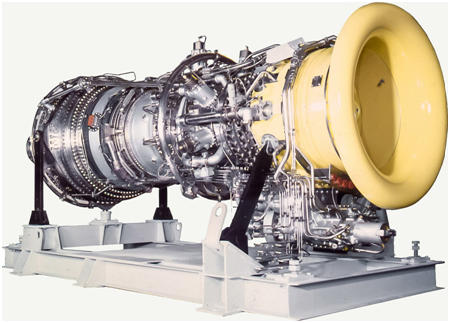
\includegraphics[scale=1]{./pictures/GTE-16PA.png}
        \caption{Фотография установки ГТЭ-16ПА.}
        \label{pic_gte_16pa}
    \end{figure}

    Газотурбинная установка ГТЭ-16ПА (рис.~\ref{pic_gte_16pa}) создана на базе двигателя ПС-90ЭУ-16А.
    Этот новый двигатель разработан в рамках сотрудничества ОАО «Авиадвигатель» с фирмой Pratt\&Whitney (США).
    Установка выполнена по двухвальной схеме с силовой турбиной.
    Она состоит из 14-ти ступенчатого осевого компрессора, камеры сгорания, 2-х ступенчатой турбины
    компрессора и 4-х ступенчатой силовой турбины.
    Эффективный КПД установки составляет 36,6\%~\cite{aviadvig}.
    С целью повышения эксплуатационной технологичности и экологической безопасности на двигатель
    устанавливается система электрозапуска.
    Главным конструктивным отличием ПС-90ЭУ-16А от других промышленных двигателей, разработанных
    ОАО «Авиадвигатель» за последние 12-13 лет, является четырехступенчатая свободная силовая турбина с номинальной
    частотой вращения 3000 об/мин~\cite{gtes-16pa}.
    Выходной вал является приводом синхронного турбогенератора Т-16-2РУХЛ3 производства ОАО «Привод» (г. Лысьва).
    Уменьшение частоты оборотов дает возможность отказаться от использования редуктора, снизив тем самым
    эксплуатационные затраты и повысив надежность всей газотурбинной установки в целом.
    Вместо оптимальной по аэродинамике пятиступенчатой силовой турбины было принято решение о
    проектировании четырехступенчатой.
    Увеличение аэродинамической нагрузки на ступень и снижение примерно на 1\% КПД силовой турбины от максимально
    достижимой величины позволило заведомо снизить суммарные затраты потенциальных заказчиков почти на 20\%~\cite{raz_konstr_perm}
    Для снижения материалоемкости и веса ГТЭ-16ПА был использован богатый опыт разработки авиационных турбин.
    В результате масса ротора двигателя ПС-90ЭУ-16А, несмотря на увеличение диаметра и количества ступеней,
    оказалась равной массе ротора ПС-90ГП-2, что позволило обеспечить высокую степень унификации трансмиссий.~\cite{raz_konstr_perm}


    \paragraph{Установка SGT-500.}

    \begin{figure}[h!]
        \centering
        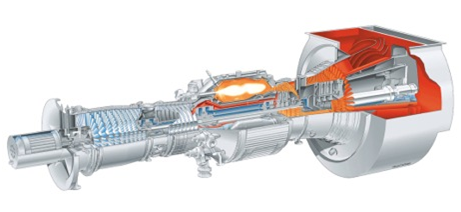
\includegraphics[scale=1.0]{./pictures/SGT-500.png}
        \caption{Схема установки SGT-500.}
        \label{pic_stg_500}
    \end{figure}

    SGT-500 (GT35C) (рис.~\ref{pic_stg_500}) мощностью 17 МВт применяется на различных объектах, где наиболее важными параметрами
    являются: базовая нагрузка, способность работать на различных видах  топлива, простота технического
    обслуживания.
    Наряду с производством  электроэнергии, SGT-500 широко используется как механический
    привод  мощностью 23290 л.с. Может работать на различных видах тяжелого топлива.
    Относительно невысокая температура газов перед турбиной способствует снижению деградации характеристик и
    увеличению межремонтного ресурса ГТУ (80 000 ч), а модульный принцип конструкции позволяет
    быстро производить замену узлов.
    Модульная и компактная конструкция турбины SGT-500 облегчает обслуживание на месте — можно быстро менять целые модули.
    В турбине SGT-500 установлен двухвальный газогенератор: на валу низкого давления установлен
    10-ступенчатый компрессор низкого давления и 2-ступенчатая турбина низкого давления.
    На валу высокого давления установлен 8-ступенчатый компрессор высокого давления и
    1-ступенчатая турбина высокого давления.
    Обороты трехступенчатой турбины равны 3600 мин-1 при генерации электроэнергии и 3450 мин-1 при
    приводе механических устройств.
    Для повышения эффективности между статором и ротором
    силовой турбины устанавливается регулятор зазора между корпусом и концами лопаток.
    Турбина поставляется с обычной системой сжигания топлива либо с системой сухого снижения
    токсичности выхлопных газов (DLE).
    Обе системы поддерживают работу на двух видах топлива, а система DLE обеспечивает крайне низкий
    уровень выбросов $NO_{x\leq}$42 ppmV.Все подшипники газодинамические,
    с шарнирно-закрепленным сегментом подпятника.
    Пусковой электродвигатель соединен с ротором компрессора низкого давления.~\cite{sgt-500}

    \paragraph{Установка Titan 130.}

    \begin{figure}[h!]
        \centering
        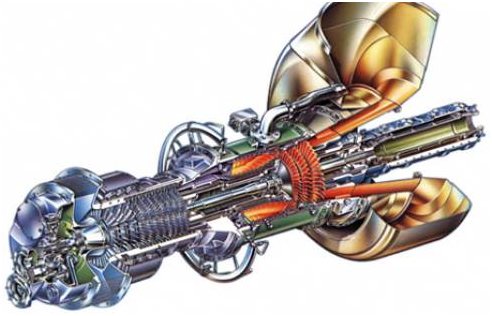
\includegraphics[scale=1.0]{./pictures/Titan_130.png}
        \caption{Схема установки Titan 130.}
        \label{pic_titan130}
    \end{figure}

    Titan 130 (рис.~\ref{pic_titan130}) – установка мощностью 16,5 МВт.
    Выполнена по одновальной схеме.
    Состоит из 14-ти ступенчатого компрессора со степенью сжатия 17,1, кольцевой камеры сгорания с
    системой сухого снижения токсичности выхлопных газов и 3-х ступенчатой силовой турбины.
    Частота вращения вала силовой турбины 11220 об/мин.
    Электрический КПД установки составляет 35,5 \%.~\cite{titan130}

    \paragraph{Установка АЛ-31СТЭ.}

    \begin{figure}[h!]
        \centering
        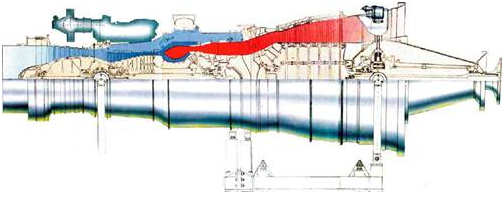
\includegraphics[scale=1.0]{./pictures/AL-31ST.png}
        \caption{Схема установки АЛ-31СТЭ.}
        \label{pic_al_31st}
    \end{figure}

    Также в классе мощности 16 МВт можно выделить двигатель АЛ-31СТЭ,
    конвертированный из двухконтурного двигателя самолета СУ-27 АЛ-31Ф.
    Схема данного двигателя представлена на рис.~\ref{pic_al_31st}.
    Данный двигатель также состоит из газогенератора и модуля свободной турбины, что облегчает ее модульный монтаж.
    Мощность на валу силовой турбины составляет 18 МВт, КПД – 38,1\%.
    Двигателю АЛ31-СТЭ свойственен невысокий по меркам стационарной техники ресурс в 75 000 ч, что
    связано с назначением двигателя – прототипа.
    Двигатель прототип АЛ-31Ф был разработан для высокоманевренного самолета СУ-27, и при его проектирование
    в основном велось на условие максимизации тяги.
    Низкоэмиссионная камера сгорания установки обеспечивает уровень вредных выбросов оксида азота
    менее 40 ppm и оксида углерода менее 80 ppm.
    Высокое совершенство рабочего процесса в камере сгорания достигнуто за счет предварительного
    смешения топливного газа в модуле-гомогенизаторе и поддержания оптимальных значений коэффициентов
    избытка воздуха в первой и второй зонах горения. Окружная неравномерность поля температуры на выходе из
    камеры сгорания снижена в 2 раза по сравнению с исходной камерой сгорания.~\cite{al-31st}
    Модульная конструкция привода обеспечивает замену узлов без
    дополнительных работ по подгонке, балансировке и испытаниям.~\cite{al-31st}


    \paragraph{Установка Т16.}
    \begin{figure}[h!]
        \centering
        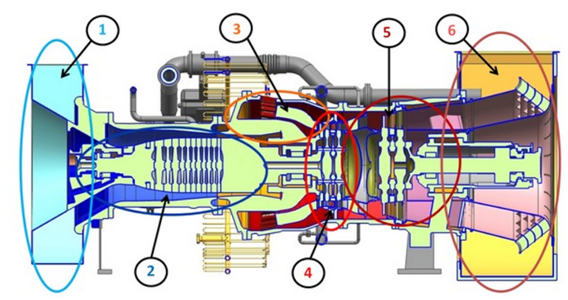
\includegraphics[scale=1.0]{./pictures/T16.png}
        \caption{Продольный разрез турбины Т16.}
        \label{pic_t16}
    \end{figure}

    Также в рассматриваемом классе мощностей присутствует одна из новейших российских газотурбинных электростанций:
    ГТЭ-16 на базе стационарной газотурбинной установки Т16 производства компании «РЭП Холдинг» в сотрудничестве с
    GEOil\&Gas.

    Схема установки представлена на рис.~\ref{pic_t16}.
    Данная установка конструктивно выполнена по двухвальной схеме со свободной турбиной.
    Отличительной особенностью установки является высокий ресурс (200 000 ч) ~\cite{rep_holding} при высоком значении КПД (37 \%)
    и низком уровне эмиссии оксидов азота (менее 25 ppm)~\cite{turbineT16}.
    Камера сгорания выполнена по противоточной схеме.
    Для поддержания высокого КПД на режимах частичной мощности (от 20\% до 100\% номинальной мощности)
    применяются поворотные направляющие аппараты трех ступеней компрессора, а также поворотный сопловой
    аппарат первой ступени силовой турбины~\cite{turbineT16}.
    Модули высокого и низкого давления располагаются на отдельных рамах и монтируются в корпусе на
    подвижных опорах, что позволяет извлекать их из общего корпуса установки в боковом направлении
    (рис.~\ref{pic_t16_tb_roll_out}-~\ref{pic_t16_pt_roll_out}) по отдельности или совместно.
    Такое конструктивное решение значительно упрощает обслуживание установки~\cite{turbineT16}.

    \begin{figure}[h!]
        \centering
        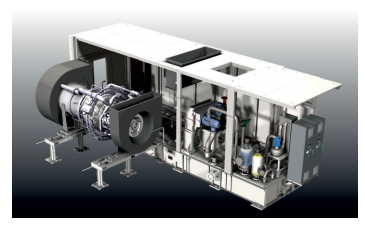
\includegraphics[scale=1.0]{./pictures/T16_tb_roll-out.png}
        \caption{Выкатка турбоблока целиком.}
        \label{pic_t16_tb_roll_out}
        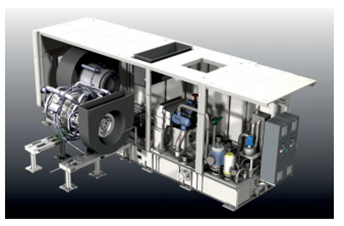
\includegraphics[scale=1.0]{./pictures/T16_gg_roll-out.png}
        \caption{Выкатка газогенератора.}
        \label{pic_t16_gg_roll_out}
        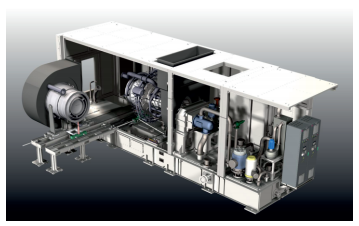
\includegraphics[scale=1.0]{./pictures/T16_pt_rool-out.png}
        \caption{Выкатка модуля силовой турбины.}
        \label{pic_t16_pt_roll_out}
    \end{figure}


    \subsection{Выбор схемы и параметров проектируемой ГТУ.}

    \begin{longtable}{|p{3.5cm}|p{2.2cm}|p{2.2cm}|p{2.2cm}|p{2.2cm}|p{2.2cm}|}

            \caption{Параметры различных установок в классе мощности 16 МВт.}\\

            \hline \label{engines16MW}
            Установка & ГТЭ-16ПА & SGT-500 & Titan 130 & АЛ-31СТЭ & T16 \\
            \hline
            Производитель & АО «ОДК-Пермские моторы» & Siemens & Solar Turbines Inc. & ПАО «ОДК-УМПО» & АО «РЭП Холдинг» \\
            \hline
            Мощность на валу силовой турбины, МВт &	16,8 & 19,7 & 16,96 &18 & 16,5 \\
            \hline
            Эффективный КПД, \% &	36,6 &	34,7 &	36,6 &	38,1 &	37,0 \\
            \hline
            Мощность на валу клеммах генератора, МВт & 16,3 &	19,1 &	16,45 &	17,46 &	16 \\
            \hline
            Электрический КПД, \% &	35,5 &	33,7 &	35,5 &	37 &	35,86 \\
            \hline
            Схема &	2Н &	3Н &	1Б &	3Н &	2Н \\
            \hline
            Степень повышения давления в компрессоре &	19,9 & 13 & 17,1 & \_ &	19,0 \\
            \hline
            Температура выхлопных газов, $^\circ C$ &	481 &	369 &	490 &	515 &	490 \\
            \hline
            Расход выхлопных газов, кг/с &	56,3 &	97,9 &	54,7 &	67 &	54,3 \\
            \hline
            Частота вращения силовой турбины, об/мин &	3000 &	3600 &	11220 &	3000 &	7800 \\
            \hline
            Температура газа перед турбиной, $^\circ C$ &	1410 &	1150 &	1400 &	\_ &	1410 \\
            \hline
            Число ступеней компрессора &	14 &	10+8 &	14 &	4+10 &	12 \\
            \hline
            Число ступеней турбины &	2+3 &	1+2+3 &	3 &	1+1+5 &	2+2 \\
            \hline
            Ресурс до капитального ремонта, ч & 20000 & 80000 & \_ & 25000 & \_ \\
            \hline
            Назначенный ресурс, ч & 100000 & 160000 & \_ & 75000 & 200000 \\
            \hline
        \end{longtable}

    Как видно из таблицы ~\ref{engines16MW} максимальный уровень температур газа для установок рассматриваемого
    класса мощности находится в районе 1400 К.
    Большинство установок, как конвертированные из авиационных, так и вновь создаваемые установки энергетического
    назначения (T16), выполнено по двухвальной схеме со свободной турбиной.
    Для перспективной установки целесообразно выбрать такую же схему, но большую начальную температуру газа,
    так как ее увеличение при заданной мощности позволяет добиться меньшего расхода рабочего тела, а, следовательно,
    и меньших диаметральных размеров, что, в свою очередь, означает уменьшнение массы.
    Также увеличение температуры газа после камеры сгорания ведет к росту эффективного КПД установки.
    Для проектируемой установки было выбрано значение начальной температуры газа $T_г^* = << comb_chamber.T_stag_out >>\ К$.
    Это выше, чем у конкурентов.
    Поэтому вышеуказанные преимущества будут обеспечены.
    Но при этом возникнет необходимость проектирования более эфективной системы охлаждения, а
    возможно и применения более эффективных защитных покрытий и жаростойких материалов для лопаточных
    аппаратов турбины.
    Это несколько увеличивает стоимоть ГТУ, но как показывает опыт, несмотря на это, удельная стоимость установки
    при увеличении температуры газа при принятых методах охлаждения существенно снижается ~\cite{manushin_eliseev_proektirovanie}.

    \newpage

    \section{Расчетно-конструкторская часть}

    \subsection{Расчет цикла установки.}

    \subsubsection{Параметры электрогенератора.}

%    << Equip.generator_params(N_gen, eta_gen, name_gen) >>

    \subsubsection{Исходные данные для расчета цикла.}
%    << TwoN.init_data(atm, inlet, comp, sink, comb_chamber, turb_c, source, turb_p, outlet, load) >>

    \subsubsection{Вариантные расчеты и выбор параметров.}
    Для выбора степени повышения давления и обоснования выбора начальной температуры газа была проведена серия расчетов
    для различных значений $\pi_к^*$ в цикле при трех различных значениях $T_г^*$: выбранном, на 50 К больше и на 50 К
    меньше выбранного.
    В результате были получены зависимости удельного расхода топлива $C_e$, эффективного КПД $\eta_e$ и расхода
    воздуха на входе в компрессор $G_в$ и мощности, отнесенной к расходу в компрессоре, $\bar{N}_e$
    от степени повышения давления в компрессоре.
    Данные зависимости предствлены на рис.~\ref{cycle_eta},~\ref{cycle_C_e},~\ref{cycle_N_e_sp},~\ref{cycle_G_air}.
    Также была произведена оценка наименьших размеров лопаточных аппаратов.
    Для турбины - это размер лопатки СА первой ступени турбины компрессора, для компрессора - размер лопатки
    последней ступени.
    Размер СА и средний диаметр турбины компрессора на входе представлены на рис.~\ref{cycle_l_sa1} и~\ref{cycle_D_av1}.

    \begin{figure}[h!]
        \centering
        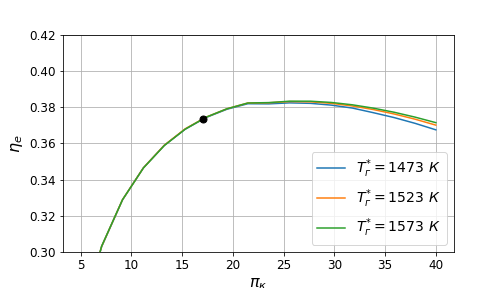
\includegraphics[scale=0.8]{../plots/cycle_eta_e.png}
        \caption{Зависимость КПД цикла от степени повышения давления.}
        \label{cycle_eta}

        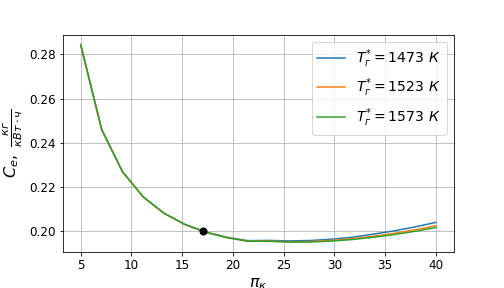
\includegraphics[scale=0.8]{../plots/cycle_C_e.png}
        \caption{Зависимость удельного расхода топлива в цикла от степени повышения давления.}
        \label{cycle_C_e}
    \end{figure}

    \begin{figure}[h!]
        \centering
        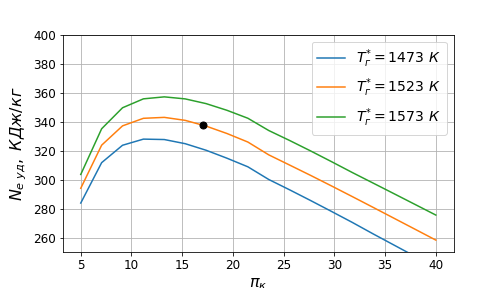
\includegraphics[scale=0.8]{../plots/cycle_N_e_sp.png}
        \caption{Зависимость удельной мощности от степени повышения давления.}
        \label{cycle_N_e_sp}

        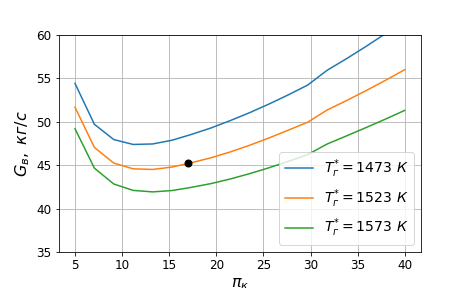
\includegraphics[scale=0.8]{../plots/cycle_G_air.png}
        \caption{Зависимость расхода воздуха на входе от степени повышения давления.}
        \label{cycle_G_air}
    \end{figure}

    \begin{figure}[h!]
        \centering
        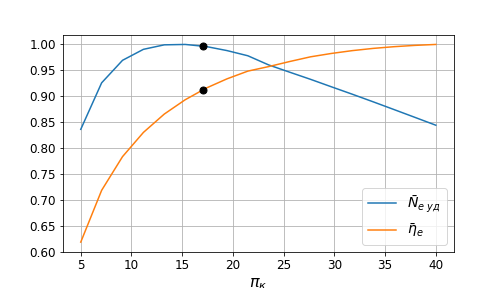
\includegraphics[scale=0.8]{../plots/cycle_N_e_sp_rel_eta_e_rel.png}
        \caption{Зависимости КПД и удельной мощности в относительных координатах от степени повышения давления.}
        \label{cycle_N_e_sp_rel_eta_e_rel}

        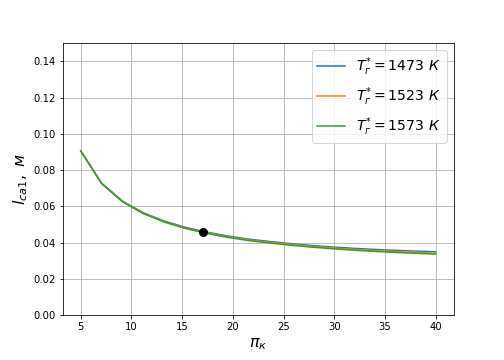
\includegraphics[scale=0.8]{../plots/cycle_l_sa1.png}
        \caption{Зависимость длина лопатки СА первой ступени турбины компрессора от степени повышения давления.}
        \label{cycle_l_sa1}
    \end{figure}

    \begin{figure}[h!]
        \centering
        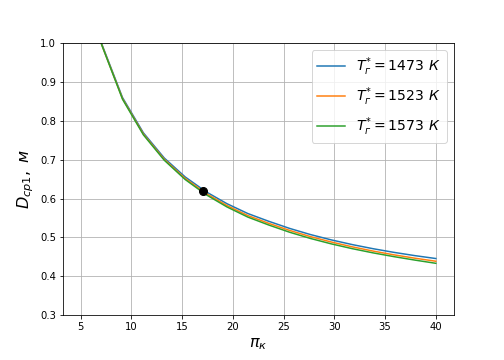
\includegraphics[scale=0.8]{../plots/cycle_D_av1.png}
        \caption{Зависимость среднего диаметра на входе в турбину компрессора от степени повышения давления.}
        \label{cycle_D_av1}
    \end{figure}

    С точки зрения максимального уменьшения диаметральных размеров лопаточных машин необходимо выбрать
    значение $pi_к^*$, соответствующее минимуму расхода воздуха $G_в$ или максимуму удельной мощности $\bar{N}_e$.
    При этом данное значение не будет оптимальным с точки зрения экономичности.
    Как видно по графику максимум по КПД находится в райное $\pi_к^* \sim 35$.
    Выбирать такие значения $\pi_к^*$ с точки зрения металлоемкости крайне невыгодно, так они далеки от оптимума
    по расходу, а также потому, что увеличение $\pi_к^*$ приводит к увеличению числа ступеней, а, стало быть, и
    росту металлоемости.
    В виду данных соображений наиболее предпочтительно выбрать значение $\pi_к^*$ в промежутке между оптимумами
    по расходу и КПД, но ближе к оптимуму по расходу, чтобы выиграть в КПД но практически не проиграть по расходу,
    так как в районе оптимума по расходу функция $G_в = f(\pi_к^*)$ очень пологая.
    Таким образом, для проектирумой установки было выбрно значение степени повышеня давления $\pi_к^* = <<comp.pi_c>>$.

    \subsubsection{Расчет цикла на номинальном режиме.}
%    << TwoN.cycle(atm, inlet, comp, sink, comb_chamber, turb_c, source, turb_p, outlet, load) >>

    \subsubsection{Параметры дожимного компрессора.}

%    << Equip.gas_compressor_params(N_gen, N_gas_comp, mass_rate_gas_comp, press_in_gas_comp, press_out_gas_comp, T_in_gas_comp, T_out_gas_comp, rho_gas_comp, c_p_nat_gas_av, k_nat_gas_av, eta_ad_gas_comp, eta_el_eng, name_gas_comp) >>

    \subsection{Расчет компрессора.}
    В данном разделе будут приведены результаты поступенчатого расчета компрессора проектируемой установки
    по средней линии тока и пример расчета для первой ступени, так как расчет каждой ступени совершается
    по одинаковой методике.
    Расчет произведен по методике изложенной в ~\cite{beknev_comp}.
    \subsubsection{Результаты поступенчатого расчета.}
%    << comp_avline_temp.stage_tables(comp_avline) >>
    \subsubsection{Исходные данные для расчета первой ступени.}
%    << comp_avline_temp.stage_init_data(comp_avline[0]) >>
    \subsubsection{Расчет первой ступени.}
%    << comp_avline_temp.stage(comp_avline[0]) >>

    \subsection{Расчет турбины компрессора.}
    В данном разделе представлен поступенчатый газодинамический расчет турбины компрессора по средней линии тока.
    Также описана методика расчета параметров потока по высоте ступени и представлены результаты расчета параметров
    потока по высоте для обоих ступеней турбины.
    Расчет выполнен по методике, изложенной в ~\cite{molyakov1} и ~\cite{molyakov2}
    \subsubsection{Результаты поступенчатого расчета.}
%    << turb_avline_temp.stage_tables(comp_turb_avline) >>
    \subsubsection{Исходные данные для расчета первой ступени.}
%    << turb_avline_temp.stage_init_data(comp_turb_avline[0], 'heat_drop') >>
    \subsubsection{Расчет первой ступени.}
%    << turb_avline_temp.heat_drop_stage(comp_turb_avline[0]) >>
    \subsubsection{Исходные данные для расчета второй ступени.}
%    << turb_avline_temp.stage_init_data(comp_turb_avline[1], 'work') >>
    \subsubsection{Расчет второй ступени.}
%    << turb_avline_temp.work_stage(comp_turb_avline[1]) >>
    \subsubsection{Расчет интегральных параметров турбины.}
%     </ set L_t_sum_exp = ((comp_turb_avline[0].L_t_prime / 10**6) | round(4)).__str__() + '\cdot 10^6' + '+' + ((comp_turb_avline[1].L_t_prime / 10**6) | round(4)).__str__() + '\cdot 10^6' />
%    << turb_avline_temp.integrate_turbine_param(comp_turb_avline, L_t_sum_exp) >>
    \subsubsection{Расчет параметров потока по высоте.}
%    << turb_prof_temp.rad_dist_alg() >>
%    << turb_prof_temp.rad_dist_res(comp_turb_st1_params, 'Параметры первой ступени на различных радиусах.', 'const_angle') >>
%    << turb_prof_temp.rad_dist_res(comp_turb_st2_params, 'Параметры второй ступени на различных радиусах.', 'const_angle') >>

    \subsection{Расчет силовой турбины.}
    В данном разделе представлен поступенчатый газодинамический расчет силовой турбины по средней линии тока.
    Расчет выполнен по методике, изложенной в ~\cite{molyakov1} и ~\cite{molyakov2}
    \subsubsection{Результаты поступенчатого расчета.}
%    << turb_avline_temp.stage_tables(power_turb_avline) >>
    \subsubsection{Исходные данные для расчета первой ступени.}
%    << turb_avline_temp.stage_init_data(power_turb_avline[0], 'heat_drop') >>
    \subsubsection{Расчет первой ступени.}
%    << turb_avline_temp.heat_drop_stage(power_turb_avline[0]) >>
    \subsubsection{Исходные данные для расчета второй ступени.}
%    << turb_avline_temp.stage_init_data(power_turb_avline[1], 'work') >>
    \subsubsection{Расчет второй ступени.}
%    << turb_avline_temp.work_stage(power_turb_avline[1]) >>
    \subsubsection{Расчет интегральных параметров турбины.}
%     </ set L_t_sum_exp = ((power_turb_avline[0].L_t_prime / 10**6) | round(4)).__str__() + '\cdot 10^6' + '+' + ((power_turb_avline[1].L_t_prime / 10**6) | round(4)).__str__() + '\cdot 10^6' />
%    << turb_avline_temp.integrate_turbine_param(power_turb_avline, L_t_sum_exp) >>

    \subsection{Расчет камеры сгорания.}

    \subsubsection{Исходные данные.}
%    << comb_geom_templ.init_data(comb_geom) >>
    \subsubsection{Расчет.}
%    << comb_geom_templ.calc(comb_geom) >>

    \section{Научно-исследовательская часть.}
    \subsection{Расчет конвективно-пленочной системы охлаждения СА первой ступени турбины компрессора.}
    \subsubsection{Описание алгоритма расчета температурного поля лопатки.}
%    << turb_cool_temp.description() >>
    \subsubsection{Методика расчета пленки.}
%    << turb_cool_temp.film() >>
    \subsubsection{Методика расчета температуры охлаждающего воздуха.}
%    << turb_cool_temp.air_temp() >>
    \subsubsection{Методика расчета температуры стенки.}
%    << turb_cool_temp.wall_temp() >>
    \subsubsection{Результаты расчета для наиболее горячего сектора.}
%    << turb_cool_temp.sector_params(cool_film_params, caption='Значения параметров в отверстиях.') >>
%    << turb_cool_temp.sector_params(cool_local_params, caption='Значения локальных параметров.') >>
    \subsubsection{Интегральные параметры охлаждения.}
%    << turb_cool_temp.integrate_params(cool_results, comp_turb_st1_sa_blade_num, comp_avline.G) >>


    \subsection{Расчет переменных режимов работы установки.}

    \section{Технологическая часть.}
    \section{Организационно-экономическая часть.}
    \section{Экология и промышленная безопасность.}

    \section{ЗАКЛЮЧЕНИЕ}

    \newpage
    \begin{thebibliography}{40}

        \bibitem{aviadvig}
%        Для энергетики [Электронныйресурс]. // Авиадвигатель.URL: \url{http://www.avid.ru/energy/}. (Дата обращения: 15.10.2017).

        \bibitem{gtes-16pa}
%        ГТЭС-16ПА [Электронныйресурс]. //
%        Тригенерация.ру.URL: \url{http://www.combienergy.ru/katalog/1-Gazoturbinnye-elektrostancii-GTES-kogeneracionnogo-cikla/83-GTES-16PA}.
%        (Дата обращения: 15.12.2017).

        \bibitem{raz_konstr_perm}
%        Рациональное конструирование - в соответствии с требованиями заказчика [Электронныйресурс].
%        // Пермские моторы.URL: \url{http://www.pmz.ru/pr/other/ntex/ib4e/konstruir/}.(Дата обращения: 15.12.2017).

        \bibitem{sgt-500}
%        Газовая турбина SGT-500 [Электронныйресурс]. //
%        Siemens.URL: \url{https://www.energy.siemens.com/ru/ru/fossil-power-generation/gas-turbines/sgt-500.htm#content=%D0%9E%D0%BF%D0%B8%D1%81%D0%B0%D0%BD%D0%B8%D0%B5}.(Дата обращения: 15.12.2017).

        \bibitem{titan130}
%        Titan 130 [Электронныйресурс]. // SolarTurbines.URL:
%        \url{https://mysolar.cat.com/en_US/products/oil-and-gas/gas-turbine-packages/generator-sets/titan-130.html}.(Дата обращения: 15.12.2017).

        \bibitem{turbineT16}
%        Спирин В.В., Ерохин С.К., Чернобровкин А.А. Передодовая газовая турбина Т16 –
%        новая разработка «РЭП Холдинга» и GEOil\&Gas// Турбины и дизели.
%        Электрон. журн. 2016. №5. Режим доступа:
%        \url{https://www.reph.ru/upload/iblock/060/t16-final.pdf} (дата обращения 24.12.2017).

        \bibitem{rep_holding}
%        Энергетика энергетика[Электронныйресурс]. // РЭП Холдинг:
%        \url{http://www.reph.ru/production/energetic/}. (Дата обращения: 15.10.2017).

        \bibitem{al-31st}
%        АЛ-31СТ. Газотурбинный привод. [Электронный ресурс]. //
%        Федеральный информационный фонд отечественных и иностранных каталогов промышленной продукции.
%        URL: \url{http://промкаталог.рф/PublicDocuments/01-0786-00.pdf}.(Дата обращения: 15.12.2017).

        \bibitem{manushin_eliseev_proektirovanie}
%        Теория и проектирование газотурбинных и комбинированных установок: учебник для вузов /
%        Ю.С. Елисеев, Э.А. Манушин, В.Е. Михальцев и др. - 2-е изд., перераб. и доп. - М.:
%        Изд-во МГТУ им. Н.Э. Баумана, 2000 - 640 с.

        \bibitem{beknev_comp}
%        Расчет осевого компрессора. Методические указания по выполнению курсовых и дипломных проектов /
%        В.С. Бекнев - М.:
%        Изд-во МГТУ им. Н.Э. Баумана, 1981 - 37 с.

        \bibitem{molyakov1}
%        Теория и проектирование газовой турбины: Учеб. пособие по курсу «Лопаточные машины газотурбинных и
%        комбинированных установок. Газовые турбины». - Ч. 1: Теория и проектирование ступени газовой турбины /
%        Под ред. М.И. Осипова. - М.: Изд-во МГТУ им. Н.Э. Баумана. 2006. - 104 с.: ил.

        \bibitem{molyakov2}
%        Теория и проектирование газовой турбины: Учеб. пособие по курсу «Лопаточные машины газотурбинных и
%        комбинированных установок. Газовые турбины». - Ч. 2: Теория и проектирование многоступенчатой газовой турбины /
%        Под ред. М.И. Осипова. - М.: Изд-во МГТУ им. Н.Э. Баумана. 2008. - 116 с.: ил.

    \end{thebibliography}

\end{document}